\chapter{Results and Discussion}
\label{chap:results-discussion}

This chapter reports the experiments that evaluate the three research questions of Section~\ref{sec:research-objective}: whether a measurable sensor domain gap exists in the latent space of a geospatial foundation model, where it concentrates and which physical sensor difference produces it (RQ1), whether cross-architecture distillation from that model can produce a sensor-adaptive compact student (RQ2), and whether doing so is preferable to simply training the compact model on the target sensor directly (RQ3).
All the results below use the single configuration set out in Section~\ref{sec:configuration}, which is a distillation with domain-specific batch normalization, and the comparison of interest throughout is against a supervised baseline of identical architecture trained without any distillation.
With one exception, every condition reported in this chapter was run once, with a single fixed seed.
We therefore report the comparisons descriptively, as differences between training curves and between best-epoch scores, and not as statistical inferences.
The epoch-to-epoch validation variance is of the order of $0.02$ mIoU, so differences smaller than roughly $0.03$ should not be treated as resolved.
The exception is the degradation-ladder evaluation of Section~\ref{sec:ladder-results}, which we replicated over three seeds and for which the drops are reported with a measured seed-to-seed deviation.
That section is consequently the only one in this chapter whose smaller effects are resolved.

\section{Experimental Configuration}
\label{sec:configuration}

The teacher is TerraMind~\cite{jakubik2025terramind} at the \texttt{base} scale, fine-tuned on the Sentinel-2 branch of the triplet dataset (Section~\ref{sec:triplets}) for the eleven-class WorldCover LULC task~\cite{zanaga2022worldcover}, and frozen thereafter.
The student is a U-Net~\cite{ronneberger2015unet} with $9.85$\,M parameters, trained from a random initialisation, since no pre-trained weights are available for this backbone.
This is a material constraint, and we return to it in Section~\ref{sec:limitations}.
Both models consume the seven-band Blue--NIR stack under the per-domain normalization protocol of Section~\ref{sec:normalization}.

Two elements of this configuration deserve to be stated explicitly, since we arrived at both of them empirically and both of them materially change the results.

\paragraph{Domain-specific batch normalization.}
The student carries a separate set of batch-normalization~\cite{ioffe2015batchnorm} statistics and affine parameters for each sensor, with all convolutional weights shared, following Chang et al.~\cite{chang2019dsbn}.
Beyond its role as a domain-adaptation mechanism, this also corrects a train/test inconsistency that is inherent to the two-branch training scheme.
The two sensors are forwarded in separate passes, so during the training each pass is normalized by the batch statistics of its own domain, while a single shared set of running averages, which is a blend of the two domains, is what would be used at inference.
The encoder would therefore never encounter at test time the normalization under which it was optimised.

\paragraph{Class-imbalanced task loss.}
The WorldCover class prior on this dataset is severely imbalanced: the three rarest classes (snow/ice, mangroves, moss/lichen) together account for $1.2\%$ of labelled pixels but, under a macro-averaged mIoU, for $27\%$ of the metric.
Under unweighted cross-entropy the student never predicted these classes at all, scoring exactly zero IoU on them in training as well as validation, a failure to learn, not overfitting.
All the runs reported here therefore use a focal loss~\cite{lin2017focal} with $\gamma = 2$, and an inverse-square-root class weighting derived from the measured pixel frequencies, which is a milder variant of the effective-number scheme of Cui et al.~\cite{cui2019classbalanced}.

The contrastive representation-alignment objectives (Section~\ref{sec:contrastive-mechanism}) were implemented and ablated, but they are disabled in all the results below, since their weights are zero throughout.
That ablation is reported separately and it is not the subject of this chapter.

Table~\ref{tab:hyperparameters} lists the settings of both arms.
Everything the two conditions could share is held constant: architecture, initialisation, split, seed, normalization, augmentation, task loss, optimiser, schedule, and early-stopping criterion are identical, and the arms differ only in the presence of the teacher, the second sensor branch, and domain-specific normalization.

\begin{table}[htbp]
    \centering
    \label{tab:hyperparameters}
    \begin{tabular}{lll}
        \toprule
        Setting                 & KD + DSBN                                                                             & Supervised baseline \\
        \midrule
        \multicolumn{3}{l}{\emph{Shared}}                                                                                                     \\
        Student architecture    & \multicolumn{2}{l}{U-Net, 7 input bands, 32 decoder channels, $1{\times}1$ conv head}                       \\
        Initialisation          & \multicolumn{2}{l}{Random (no pre-trained weights available)}                                               \\
        Optimiser               & \multicolumn{2}{l}{AdamW}                                                                                   \\
        Learning rate           & \multicolumn{2}{l}{$1\times10^{-4}$}                                                                        \\
        Weight decay            & \multicolumn{2}{l}{$1\times10^{-4}$}                                                                        \\
        LR schedule             & \multicolumn{2}{l}{ReduceLROnPlateau, factor $0.5$, patience $5$}                                           \\
        Batch size              & \multicolumn{2}{l}{$8$ patches}                                                                             \\
        Early stopping          & \multicolumn{2}{l}{Patience $12$ on target-sensor validation IoU}                                           \\
        Model selection         & \multicolumn{2}{l}{Best target-sensor validation IoU}                                                       \\
        Task loss               & \multicolumn{2}{l}{Focal, $\gamma = 2.0$}                                                                   \\
        Class weighting         & \multicolumn{2}{l}{Inverse square-root of measured pixel frequency}                                         \\
        Augmentation            & \multicolumn{2}{l}{Joint geometric (flips, $90^{\circ}$ rotations)}                                         \\
        Random seed             & \multicolumn{2}{l}{$42$}                                                                                    \\
        Numerical precision     & \multicolumn{2}{l}{$32$-bit}                                                                                \\
        \midrule
        \multicolumn{3}{l}{\emph{Distillation-specific}}                                                                                      \\
        Teacher                 & TerraMind, frozen                                                                     & ---                 \\
        Distillation loss       & KL on logits, $T = 4.0$                                                               & ---                 \\
        Distillation applied to & All pixels, both branches                                                             & ---                 \\
        Task-loss weight        & $1.0$ target $+$ $1.0$ source                                                         & $1.0$ target        \\
        Distillation weight     & $1.0$                                                                                 & ---                 \\
        Contrastive weights     & $0$ (instance and pixel)                                                              & ---                 \\
        Domain-specific BN      & Enabled                                                                               & ---                 \\
        Sensor branches         & Two ($\Phi$-sat-2, Sentinel-2)                                                        & One ($\Phi$-sat-2)  \\
        \bottomrule
    \end{tabular}
    \caption{Training configuration for the two arms.
        Settings above the rule are identical by construction; those below apply to the distilled arm only.
    }
\end{table}

One asymmetry in this comparison is structural rather than incidental, and it should be stated alongside the table.
The distilled arm applies the task loss to both sensor views of each patch, so within one epoch it draws twice as much supervision from the same labels as the single-branch baseline does.
This is inherent to what the comparison is testing, since the baseline has no second view by definition, but it does mean that the per-epoch comparisons reported below are not matched on gradient signal, and it also contributes, alongside the forward pass of the frozen teacher, to the cost difference quantified in Section~\ref{sec:rq3-results}.

\wip{A second ablation, isolating domain-specific normalization from distillation itself, is in progress and is not reported here.
    It requires a distilled student trained with a single shared set of batch-normalization statistics, which is the condition that would separate the contribution of the domain-specific variant from that of the two-branch distillation scheme and the class-balanced loss adopted alongside it.
    Until that run completes, the attribution of the invariance results of Section~\ref{sec:rq2-results} to domain-specific normalization specifically should be read as provisional: what the results below establish is that the configuration as a whole produces the reported behaviour, not which of its components is responsible.
}

\section{Sensor Gap in TerraMind Latent Space (RQ1)}
\label{sec:rq1-results}

The first question is whether the domain gap is visible in the representation itself, and not only in the downstream accuracy.
We extracted embeddings for $800$ co-registered test patches from both sensors, and compared them under three measures: the paired cosine similarity between the two views of the same ground, the proxy $\mathcal{A}$-distance (PAD)~\cite{bendavid2010theory}, and a cross-domain probe-transfer test in which a linear classifier fitted on Sentinel-2 embeddings is applied to the $\Phi$-sat-2 embeddings of the same patches.

The teacher's representation does not transfer across the sensor pair.
The paired cosine similarity between the two views of the same ground is $0.098$, so the two sensors are close to orthogonal in its embedding space, and a linear probe fitted on its Sentinel-2 features retains only $33\%$ of its accuracy once it is applied to the $\Phi$-sat-2 features ($0.754 \rightarrow 0.250$).
Figure~\ref{fig:embeddings-paired} shows this directly: grey lines join the two sensor views of each patch, and in the teacher's projection they stretch across the entire embedding (median link length $6.15$ UMAP~\cite{mcinnes2018umap} units).

Per-layer analysis locates the gap.
PAD between the two domains is $1.90$--$1.98$ at every transformer block, including the first, on a scale bounded at $2$.
A gap that was semantic in origin would be expected to emerge in the deeper and more abstract layers, whereas one that is present from the first block points instead to low-level radiometry.
This is consistent with the spectral analysis of Section~\ref{sec:gap-measurement}, which found that the two sensors' digital numbers differ by more than an order of magnitude and that their per-band shapes differ in ways a single gain cannot reconcile.
This ordering is also the reverse of the resolution-driven account emphasised in related on-orbit work~\cite{du2025onorbitdemonstrationgeospatialfoundation}, since the $4.75$\,m ground sampling distance of $\Phi$-sat-2 is finer than Sentinel-2's.

\begin{figure}[htbp]
    \centering
    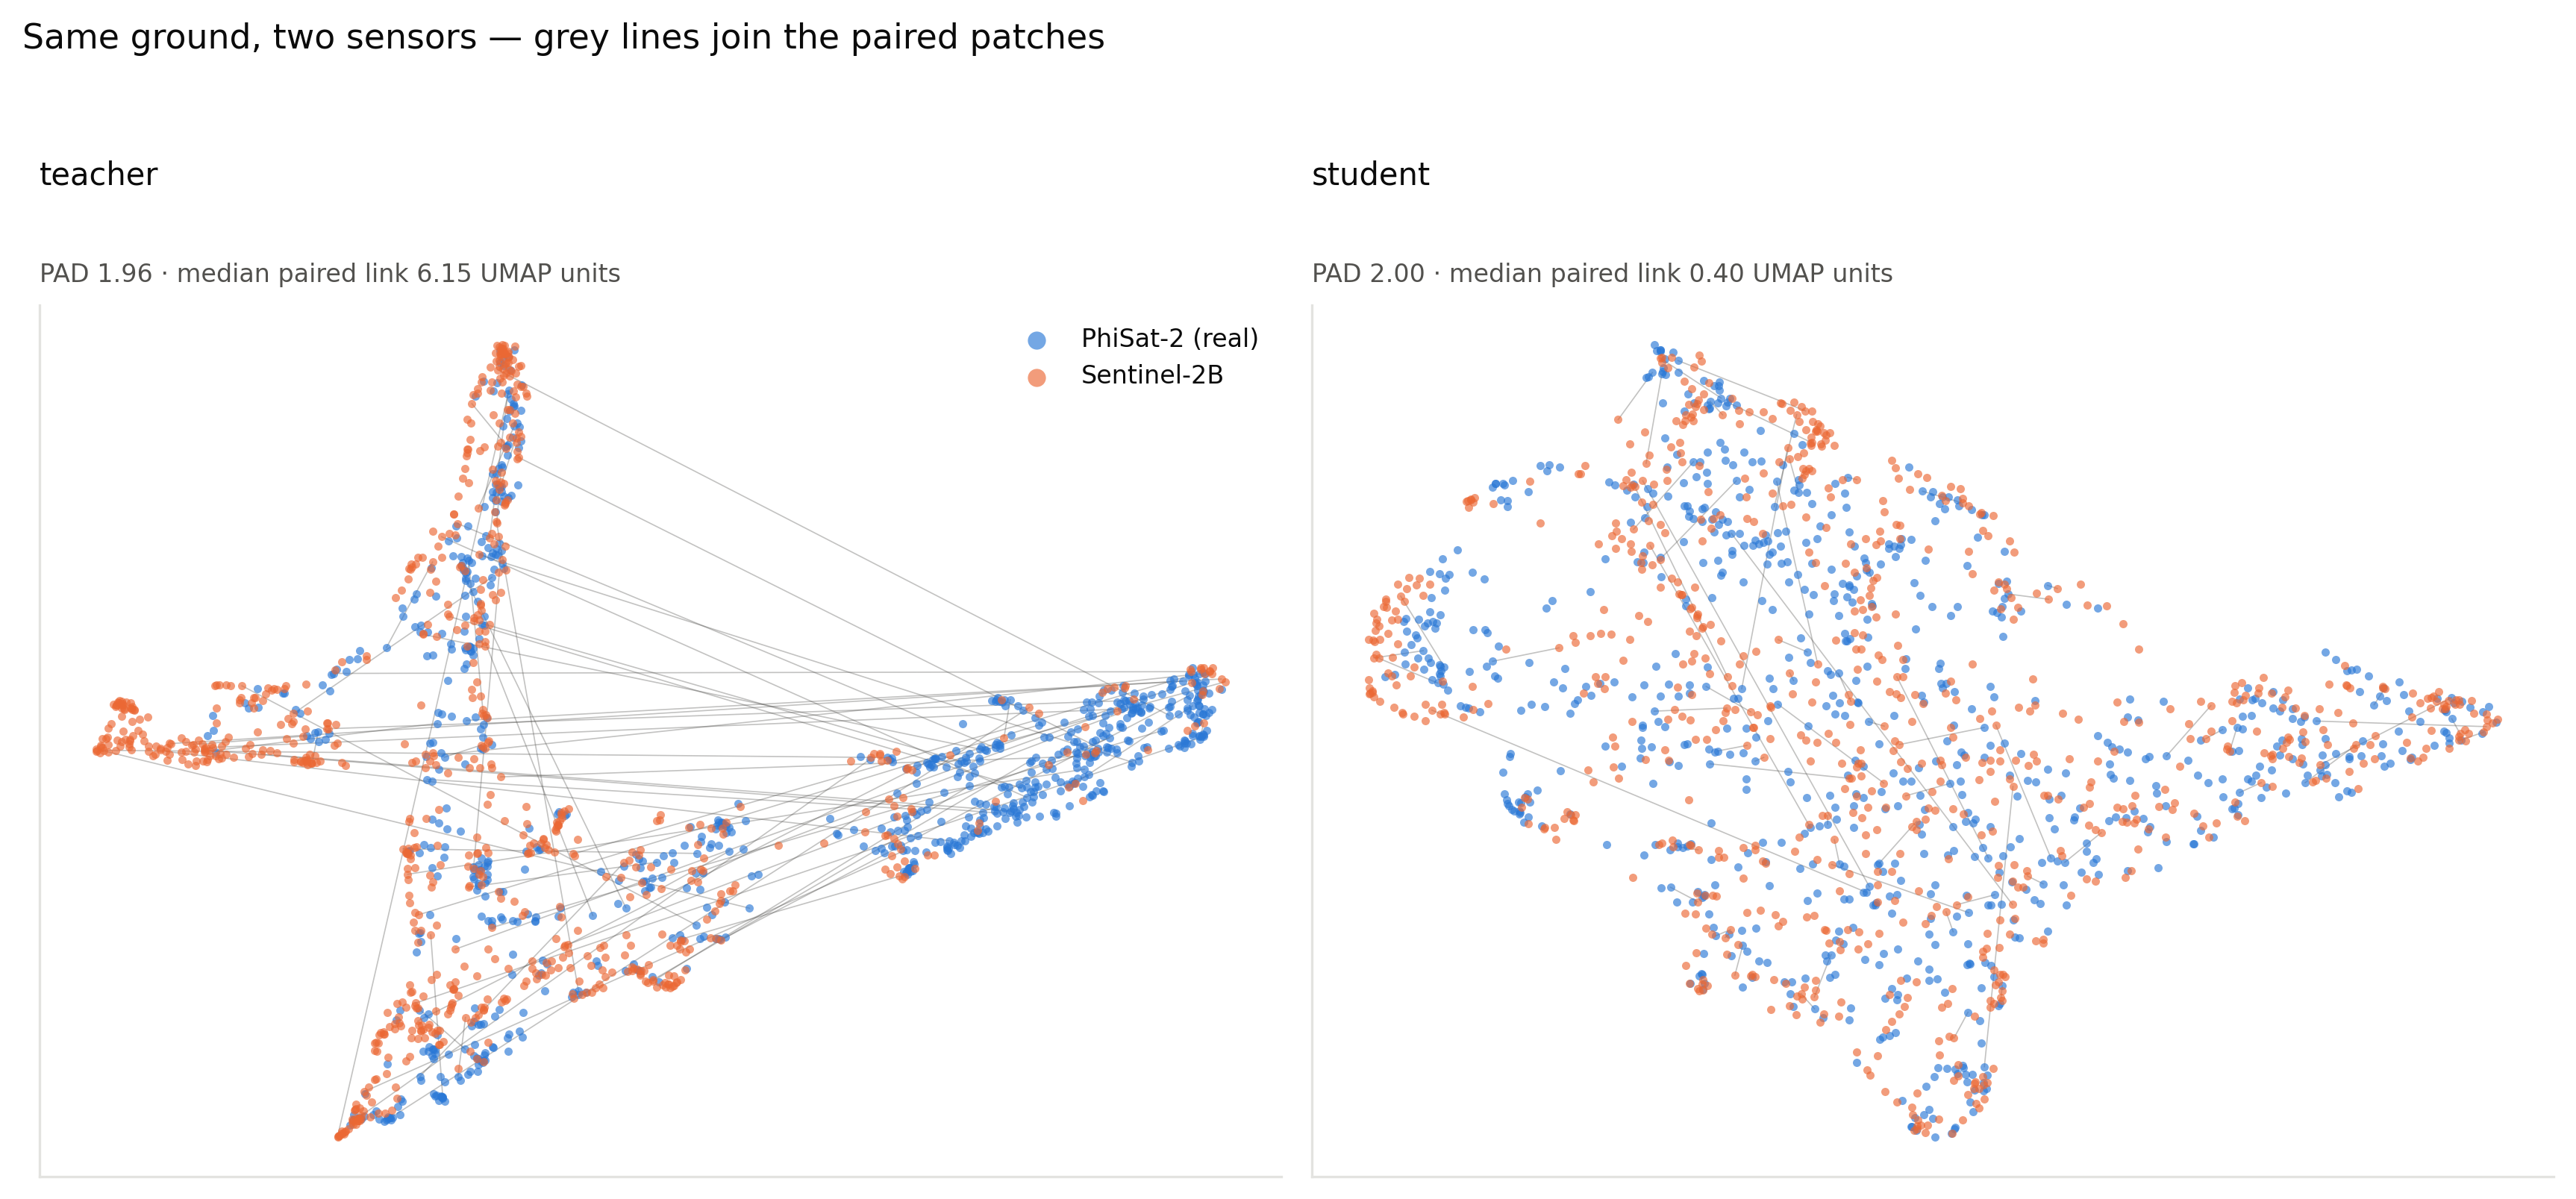
\includegraphics[width=\textwidth]{figures/fig_embeddings_paired.png}
    \caption{UMAP projection of pooled embeddings for $800$ co-registered test patches, teacher (left) and distilled student (right), each projected independently.
        Grey lines join the two sensor views of the same patch.
        In the teacher's space the paired views are far apart (median link $6.15$ units); in the student's they are effectively coincident ($0.40$ units).
    }
    \label{fig:embeddings-paired}
\end{figure}

A raw per-layer cosine-similarity check on the smaller TerraMind Tiny encoder, fine-tuned separately on real $\Phi$-sat-2 data as part of the earlier protocol described in Appendix~\ref{app:real-baseline}, is consistent with this picture (Figure~\ref{fig:cosine-sim-tiny}).
Similarity between paired Sentinel-2B and real-$\Phi$-sat-2 embeddings is near zero at the first block and rises through the middle of the network, mirroring the low-level-radiometry reading of the per-layer PAD result above.
This is a supplementary observation, on a different model scale and with a different measure than the analysis above (a raw cosine similarity in place of PAD), and we offer it as a consistency check rather than as a replication.

\begin{figure}[htbp]
    \centering
    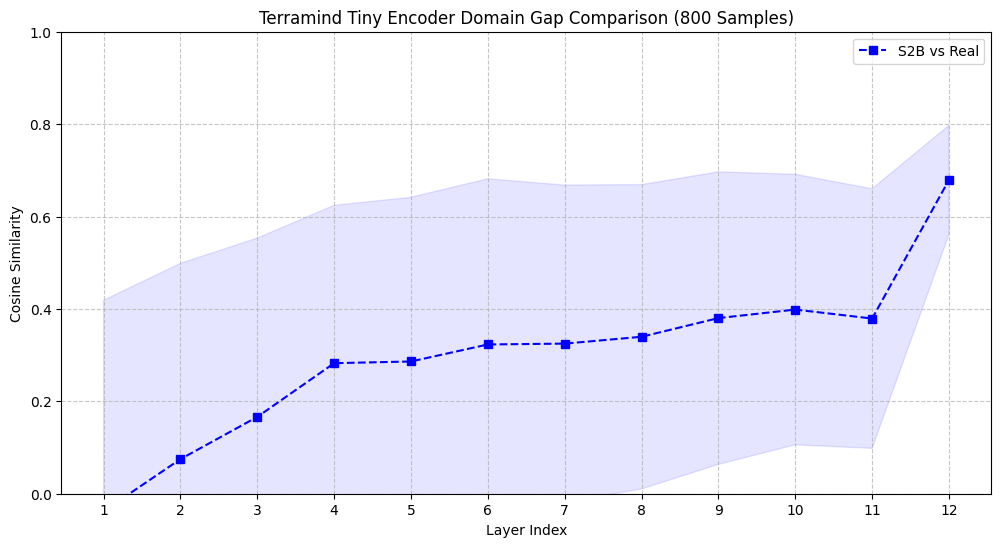
\includegraphics[width=0.85\textwidth]{figures/fig_cosine_sim_terramind.png}
    \caption{Per-layer cosine similarity between paired Sentinel-2B and real-$\Phi$-sat-2 patch embeddings from the TerraMind Tiny encoder, averaged over $800$ samples (shaded band: one standard deviation).
    }
    \label{fig:cosine-sim-tiny}
\end{figure}

\section{Degradation Factor effects on Downstream Task Gap (RQ1)}
\label{sec:ladder-results}

This section takes up the last part of RQ1, which asks which of the physical differences between the two instruments is the one that produces the gap.
This sub-question takes on the measurements above that established that a gap exists and that it is low-level in origin, and it asks which of the three low-level differences is responsible: radiometric noise, optical blur, or band misalignment.
The two instruments differ in their spectral response, their radiometric noise, their band registration and their ground sampling distance all at once, and no measurement on real pairs can separate those.
The simulated ladder of Section~\ref{sec:sen1floods-sim} makes the separation possible by degrading one factor at a time over identical scene content.
Three factors are varied over four severities each: sensor noise (SNR), optical blur (PSF), and band-to-band misalignment.
Table~\ref{tab:ladder-definition} gives the parameter values.
A severity axis common to all three is defined by setting level~4 to the operating point of the joint simulator configuration and halving the perturbation magnitude at each step down, so that a given level means the same fraction of full simulated degradation whichever factor is being varied.

\begin{table}[htbp]
    \centering
    \label{tab:ladder-definition}
    \begin{tabular}{lcccc}
        \toprule
        Level & Severity & SNR range  & PSF $\sigma$ (px) & Misalignment $\sigma$ (px) \\
        \midrule
        L1    & $0.125$  & $[40, 80]$ & $0.5$             & $1.25$                     \\
        L2    & $0.250$  & $[20, 40]$ & $1.0$             & $2.50$                     \\
        L3    & $0.500$  & $[10, 20]$ & $2.0$             & $5.00$                     \\
        L4    & $1.000$  & $[5, 10]$  & $4.0$             & $10.00$                    \\
        \bottomrule
    \end{tabular}
    \caption{The degradation ladder.
        Level~4 reproduces the joint simulator configuration; each step down halves the perturbation.
        SNR is drawn per scene from the stated range and the noise amplitude scales as its reciprocal, so the four ranges correspond to relative noise of $1/8$, $1/4$, $1/2$ and $1$.
        Blur and misalignment parameters are in resampled $4.75$\,m pixels.
    }
\end{table}

What we measure here is the domain gap proper: each model is trained once on the undegraded rung, and the resulting checkpoint is then evaluated on the test split of every rung, so the degradation only appears at inference, exactly as it would for a model trained on Sentinel-2 and deployed on $\Phi$-sat-2.
Three encoder configurations are compared: the distilled student with its encoder frozen and its decoder trained ($5.14$\,M of $9.86$\,M parameters trainable), TerraMind \texttt{base} under the same frozen-encoder protocol ($7.92$\,M of $94.25$\,M), and TerraMind \texttt{base} fine-tuned end to end.
Each configuration is run for three seeds using the same model checkpoint across all test splits.
Table~\ref{tab:ladder-domain-gap} reports the results.

\begin{table}[htbp]
    \centering
    \label{tab:ladder-domain-gap}
    \begin{tabular}{lccc}
        \toprule
                             & Distilled student           & TerraMind base            & TerraMind base                     \\
                             & (encoder frozen)            & (encoder frozen)          & (fine-tuned)                       \\
        \midrule
        Clean baseline (IoU) & $\mathbf{0.814} \pm 0.002$  & $0.739 \pm 0.057$         & $0.773 \pm 0.033$                  \\
        \midrule
        \multicolumn{4}{l}{\emph{Sensor noise (SNR)}}                                                                       \\
        \quad L1             & $-0.031 \pm 0.024$          & $+0.002 \pm 0.003$        & $-0.001 \pm 0.001$                 \\
        \quad L2             & $-0.114 \pm 0.099$          & $+0.003 \pm 0.006$        & $-0.004 \pm 0.002$                 \\
        \quad L3             & $-0.280 \pm 0.234$          & $-0.018 \pm 0.017$        & $-0.041 \pm 0.014^{\ast}$          \\
        \quad L4             & $\mathbf{-0.458} \pm 0.267$ & $-0.088 \pm 0.066$        & $-0.152 \pm 0.030^{\ast}$          \\
        \addlinespace
        \multicolumn{4}{l}{\emph{Optical blur (PSF)}}                                                                       \\
        \quad L1             & $-0.002 \pm 0.000^{\ast}$   & $-0.004 \pm 0.003$        & $0.000 \pm 0.000$                  \\
        \quad L2             & $-0.013 \pm 0.003^{\ast}$   & $-0.010 \pm 0.007$        & $0.000 \pm 0.001$                  \\
        \quad L3             & $-0.048 \pm 0.014^{\ast}$   & $-0.016 \pm 0.012$        & $0.000 \pm 0.003$                  \\
        \quad L4             & $-0.110 \pm 0.030^{\ast}$   & $-0.025 \pm 0.016$        & $\mathbf{-0.008} \pm 0.009$        \\
        \addlinespace
        \multicolumn{4}{l}{\emph{Band misalignment}}                                                                        \\
        \quad L1             & $-0.006 \pm 0.001^{\ast}$   & $-0.008 \pm 0.003^{\ast}$ & $-0.003 \pm 0.001^{\ast}$          \\
        \quad L2             & $-0.031 \pm 0.001^{\ast}$   & $-0.033 \pm 0.005^{\ast}$ & $-0.013 \pm 0.003^{\ast}$          \\
        \quad L3             & $-0.082 \pm 0.004^{\ast}$   & $-0.065 \pm 0.005^{\ast}$ & $-0.051 \pm 0.007^{\ast}$          \\
        \quad L4             & $-0.140 \pm 0.007^{\ast}$   & $-0.119 \pm 0.009^{\ast}$ & $\mathbf{-0.109} \pm 0.012^{\ast}$ \\
        \bottomrule
    \end{tabular}
    \caption{Domain gap across the degradation ladder: change in positive-class IoU relative to the undegraded test split, for a model trained only on undegraded data.
        Values are the mean over three seeds of the within-seed drop, $\pm$ one standard deviation of those drops; $^{\ast}$ marks a drop exceeding twice that deviation.
        The two model families are scored under different evaluation geometry (the student on $256$-pixel centre crops, TerraMind on full $1077$-pixel scenes), so the clean baselines are not comparable between columns and only the drops are.
    }
\end{table}

On undegraded data the distilled student is the strongest of the three, at $0.814$ IoU against $0.773$ for fine-tuned TerraMind and $0.739$ for frozen TerraMind.
The smaller student outperforming the foundation model on this clean task can be attributed to its stronger local representation, whereas TerraMind is a general-purpose encoder receiving only a task head and a fine-tuning pass.
The comparison of interest here is the response to degradation.

Band misalignment is the only factor that degrades every configuration significantly, monotonically, and by a similar amount.
Its full-severity cost varies only between $-0.109$ and $-0.140$ IoU across models that differ by an order of magnitude in trainable parameters and by architecture family, and it is the sole factor resolved at the mildest severity in all three columns, where a $1.25$-pixel shift already costs a small but reproducible amount.
Its seed-to-seed deviation is also the smallest in the table.
A perturbation whose cost is that insensitive to the model absorbing it is best read as a damage to the input signal, rather than as a weakness of any particular representation.
Band-to-band shifts corrupt precisely the cross-band relationships on which a water/land decision rests, and no amount of encoder capacity recovers an information that the shift has already destroyed.

Sensor noise produces the largest single degradation, but its magnitude is a property of the model rather than of the perturbation, and it is the least reproducible quantity in the table.
At full severity it costs the distilled student $-0.458$ IoU on average and fine-tuned TerraMind $-0.152$, a threefold difference that holds at every severity and stands in contrast to the near-constant cost of misalignment.
Neither the student's figure nor frozen TerraMind's ($-0.088$) is resolved at three seeds, because in both cases the seed-to-seed deviation of the drop ($0.267$ and $0.066$) is of the same order as the drop itself.

Optical blur is the least damaging factor in every configuration, but the three differ in how cleanly the effect is resolved.
For fine-tuned TerraMind it is indistinguishable from zero: four severities spanning a twenty-four-fold reduction in image gradient energy move the score by at most $0.008$ IoU.
For frozen TerraMind the response is monotone and uniformly negative but never clears the significance threshold, reaching $-0.025$ at full severity.
For the distilled student it is small but unambiguous, significant at all four severities with the tightest deviations in the table, rising from $-0.002$ to $-0.110$.
Blur is therefore real for the student and negligible for TerraMind, yet even for the student it remains the smallest of the three factors, costing a quarter of what noise costs at the same nominal severity.

This ordering settles the attribution question left open in Section~\ref{sec:rq1-results}, and it settles it in the same direction.
The factor that models a resolution difference, which is the optical blur, is the one that costs almost nothing, while the radiometric factor and the band-registration factor are the ones carrying the effect.
The per-layer PAD result located the gap in low-level radiometry rather than in semantics, and the ladder independently identifies the two low-level physical effects responsible, using a different task, a different measurement, and imagery in which scene content is held fixed by construction.
It also reinforces the point that the gap here is not resolution-driven, which is again the reverse of the emphasis found in related on-orbit work~\cite{du2025onorbitdemonstrationgeospatialfoundation}.

\begin{table}[htbp]
    \centering
    \label{tab:ladder-adaptation}
    \begin{tabular}{lccc}
        \toprule
        Factor at L4       & Trained clean, tested degraded & Trained and tested degraded & Recovered \\
        \midrule
        Sensor noise (SNR) & $-0.455$                       & $-0.072$                    & $84\%$    \\
        Band misalignment  & $-0.150$                       & $-0.051$                    & $66\%$    \\
        Optical blur (PSF) & $-0.128$                       & $+0.020$                    & all of it \\
        \bottomrule
    \end{tabular}
    \caption{Degradation seen at inference only, against degradation present during training as well, for the distilled student at full severity.
        The matched-condition column is a single seed and is not directly comparable in precision to the three-seed cross-condition column; it is reported to establish the size of the effect, which is large, not its exact value.
    }
\end{table}

One further comparison bears directly on what to do about these results.
Repeating the sweep with each model trained on the same degraded condition it is evaluated on, instead of on clean data, recovers most of the loss (Table~\ref{tab:ladder-adaptation}).
$84\%$ of the noise penalty and $66\%$ of the misalignment penalty disappear, and the blur ceases to be a penalty at all, since it scores marginally \emph{above} the clean baseline, in the manner of a mild augmentation.
The gap measured in Table~\ref{tab:ladder-domain-gap} is therefore largely an adaptation gap rather than an information-loss gap, at least for noise and blur.
Where the noise characteristics of the operating sensor are known in advance, which for a launched instrument they always are, simulating them during the training reclaims most of the achievable performance, and this without any domain-adaptation machinery at all.
Misalignment is again the exception: a third of its cost survives training on the degraded condition, which is consistent with reading it as genuine destruction of cross-band information.

Three limitations bound these results.
We vary the factors one at a time, whereas a real sensor pair presents all of them at once, and possibly interacting, so the ladder identifies which effects matter in isolation, and not how they compose.
The degradations are simulated, so the conclusion concerns the simulator's model of the instrument difference and not the instrument difference itself, and it is the absence of real labelled $\Phi$-sat-2 flood data (Section~\ref{sec:sen1floods-sim}) that makes this unavoidable.
Finally, the supervised U-Net baseline is not included in Table~\ref{tab:ladder-domain-gap}, so these results characterise the distilled and foundation-model encoders but do not establish whether distillation itself changed robustness relative to training on the target sensor directly.

\wip{Two further pieces of this evaluation are prepared but not yet included: a latent-space view of how the ladder displaces the U-Net's representation, and the corresponding domain-gap metrics of Section~\ref{sec:gap-measurement} computed per rung.
    Both are expected to test the same attribution from the representation side rather than the task side, and the reading above should be revisited if they disagree with it.
}

\section{Sensor Adaptivity in the Distilled Student (RQ2)}
\label{sec:rq2-results}

The distilled student inverts every one of these measurements.
The paired cosine similarity rises from $0.098$ to $0.948$, and the probe transfer from $33\%$ to $97\%$ ($0.663 \rightarrow 0.646$), which means that a classifier fitted on the student's Sentinel-2 features is very nearly as accurate on its $\Phi$-sat-2 features.
In Figure~\ref{fig:embeddings-paired} the paired links collapse to $0.40$ UMAP units, a fifteen-fold reduction.
The downstream consequence is visible in the right panel of Figure~\ref{fig:dsbn-vs-baseline}.
The accuracy of the student on the two sensors converges on parity: on the test split it scores $0.4454$ on $\Phi$-sat-2 against $0.4417$ on Sentinel-2, which is a residual difference of $-0.004$ mIoU, and this against a teacher whose representation does not usefully transfer at all.
Table~\ref{tab:invariance} collects the three measures side by side.

\begin{table}[htbp]
    \centering
    \label{tab:invariance}
    \begin{tabular}{lcc}
        \toprule
        Measure                                      & TerraMind teacher & Distilled student \\
        \midrule
        Paired cosine similarity                     & $0.098$           & $\mathbf{0.948}$  \\
        Median paired link (UMAP units)              & $6.15$            & $\mathbf{0.40}$   \\
        Probe: Sentinel-2 $\rightarrow$ Sentinel-2   & $0.754$           & $0.663$           \\
        Probe: Sentinel-2 $\rightarrow$ $\Phi$-sat-2 & $0.250$           & $\mathbf{0.646}$  \\
        Probe transfer retention                     & $33\%$            & $\mathbf{97\%}$   \\
        \addlinespace
        IoU($\Phi$-sat-2) $-$ IoU(Sentinel-2), test  & ---               & $\mathbf{-0.004}$ \\
        \bottomrule
    \end{tabular}
    \caption{Sensor invariance of the teacher and the distilled student, over $800$ co-registered test patches.
        Paired cosine and probe transfer compare the two sensor views of the \emph{same} ground.
        Probe transfer fits a linear classifier on Sentinel-2 embeddings and applies it to $\Phi$-sat-2 embeddings; retention is the ratio of the two accuracies.
        The IoU difference is measured on the full test split rather than on the $800$-patch embedding sample.
    }
\end{table}

\wip[Decide how to frame the probe row that cuts against the student.]{%
    To write: a remark on the one row that cuts against the student.
    The teacher is the stronger encoder \emph{within} Sentinel-2 ($0.754$ against $0.663$ same-domain probe accuracy), and its advantage only disappears once the probe is asked to cross the sensor gap.
    This can be framed either as a limitation of the student, or as the precise statement of what the distillation bought.
}

One measurement in this set behaves counter-intuitively, and it illustrates a real trap in evaluating this class of method.
The raw PAD is maximal for the student ($2.000$, against $1.955$ for the teacher), which means that a linear probe separates the two domains perfectly.
This is an artefact of the mechanism itself, since the domain-specific normalization gives each sensor its own affine transform.
A constant per-channel offset distinguishes the domains by construction, and a linear probe finds it trivially regardless of how well the semantic content is aligned.
Standardising each domain on its own statistics removes exactly the first and second moments that a per-domain affine can express, and it drops the probe to chance for both models.
Figure~\ref{fig:pad-decision} shows the underlying quantity: in the raw setting the two domains' probe scores are separated by an empty margin, and after per-domain standardisation they collapse onto one another.

PAD is therefore not a valid instrument for a model that carries a domain-specific normalization, even though it is scale-free and hence otherwise well suited to comparing representations of different dimensionality.
The probe transfer, which asks the functional question directly, is the appropriate measure here, and it is the one we report above.

\wip{The same caution applies in weaker form to the two measures this section does rely on.
    Domain-specific normalization aligns each domain's first and second moments by construction, and both paired cosine similarity and probe transfer are sensitive to that alignment, so some part of the improvement reported above may share an origin with the PAD artefact instead of reflecting semantic alignment alone.
    Recomputing both measures on a student trained with shared normalization, and after standardising each domain on its own statistics, is in progress and is the check that would settle how much of the gain is representational.
    Until it completes, the magnitude of the invariance improvement should be read as an upper bound, though the direction of the effect is not in doubt: the teacher's representation does not transfer across the sensor pair at all, and the student's does.
}

\begin{figure}[htbp]
    \centering
    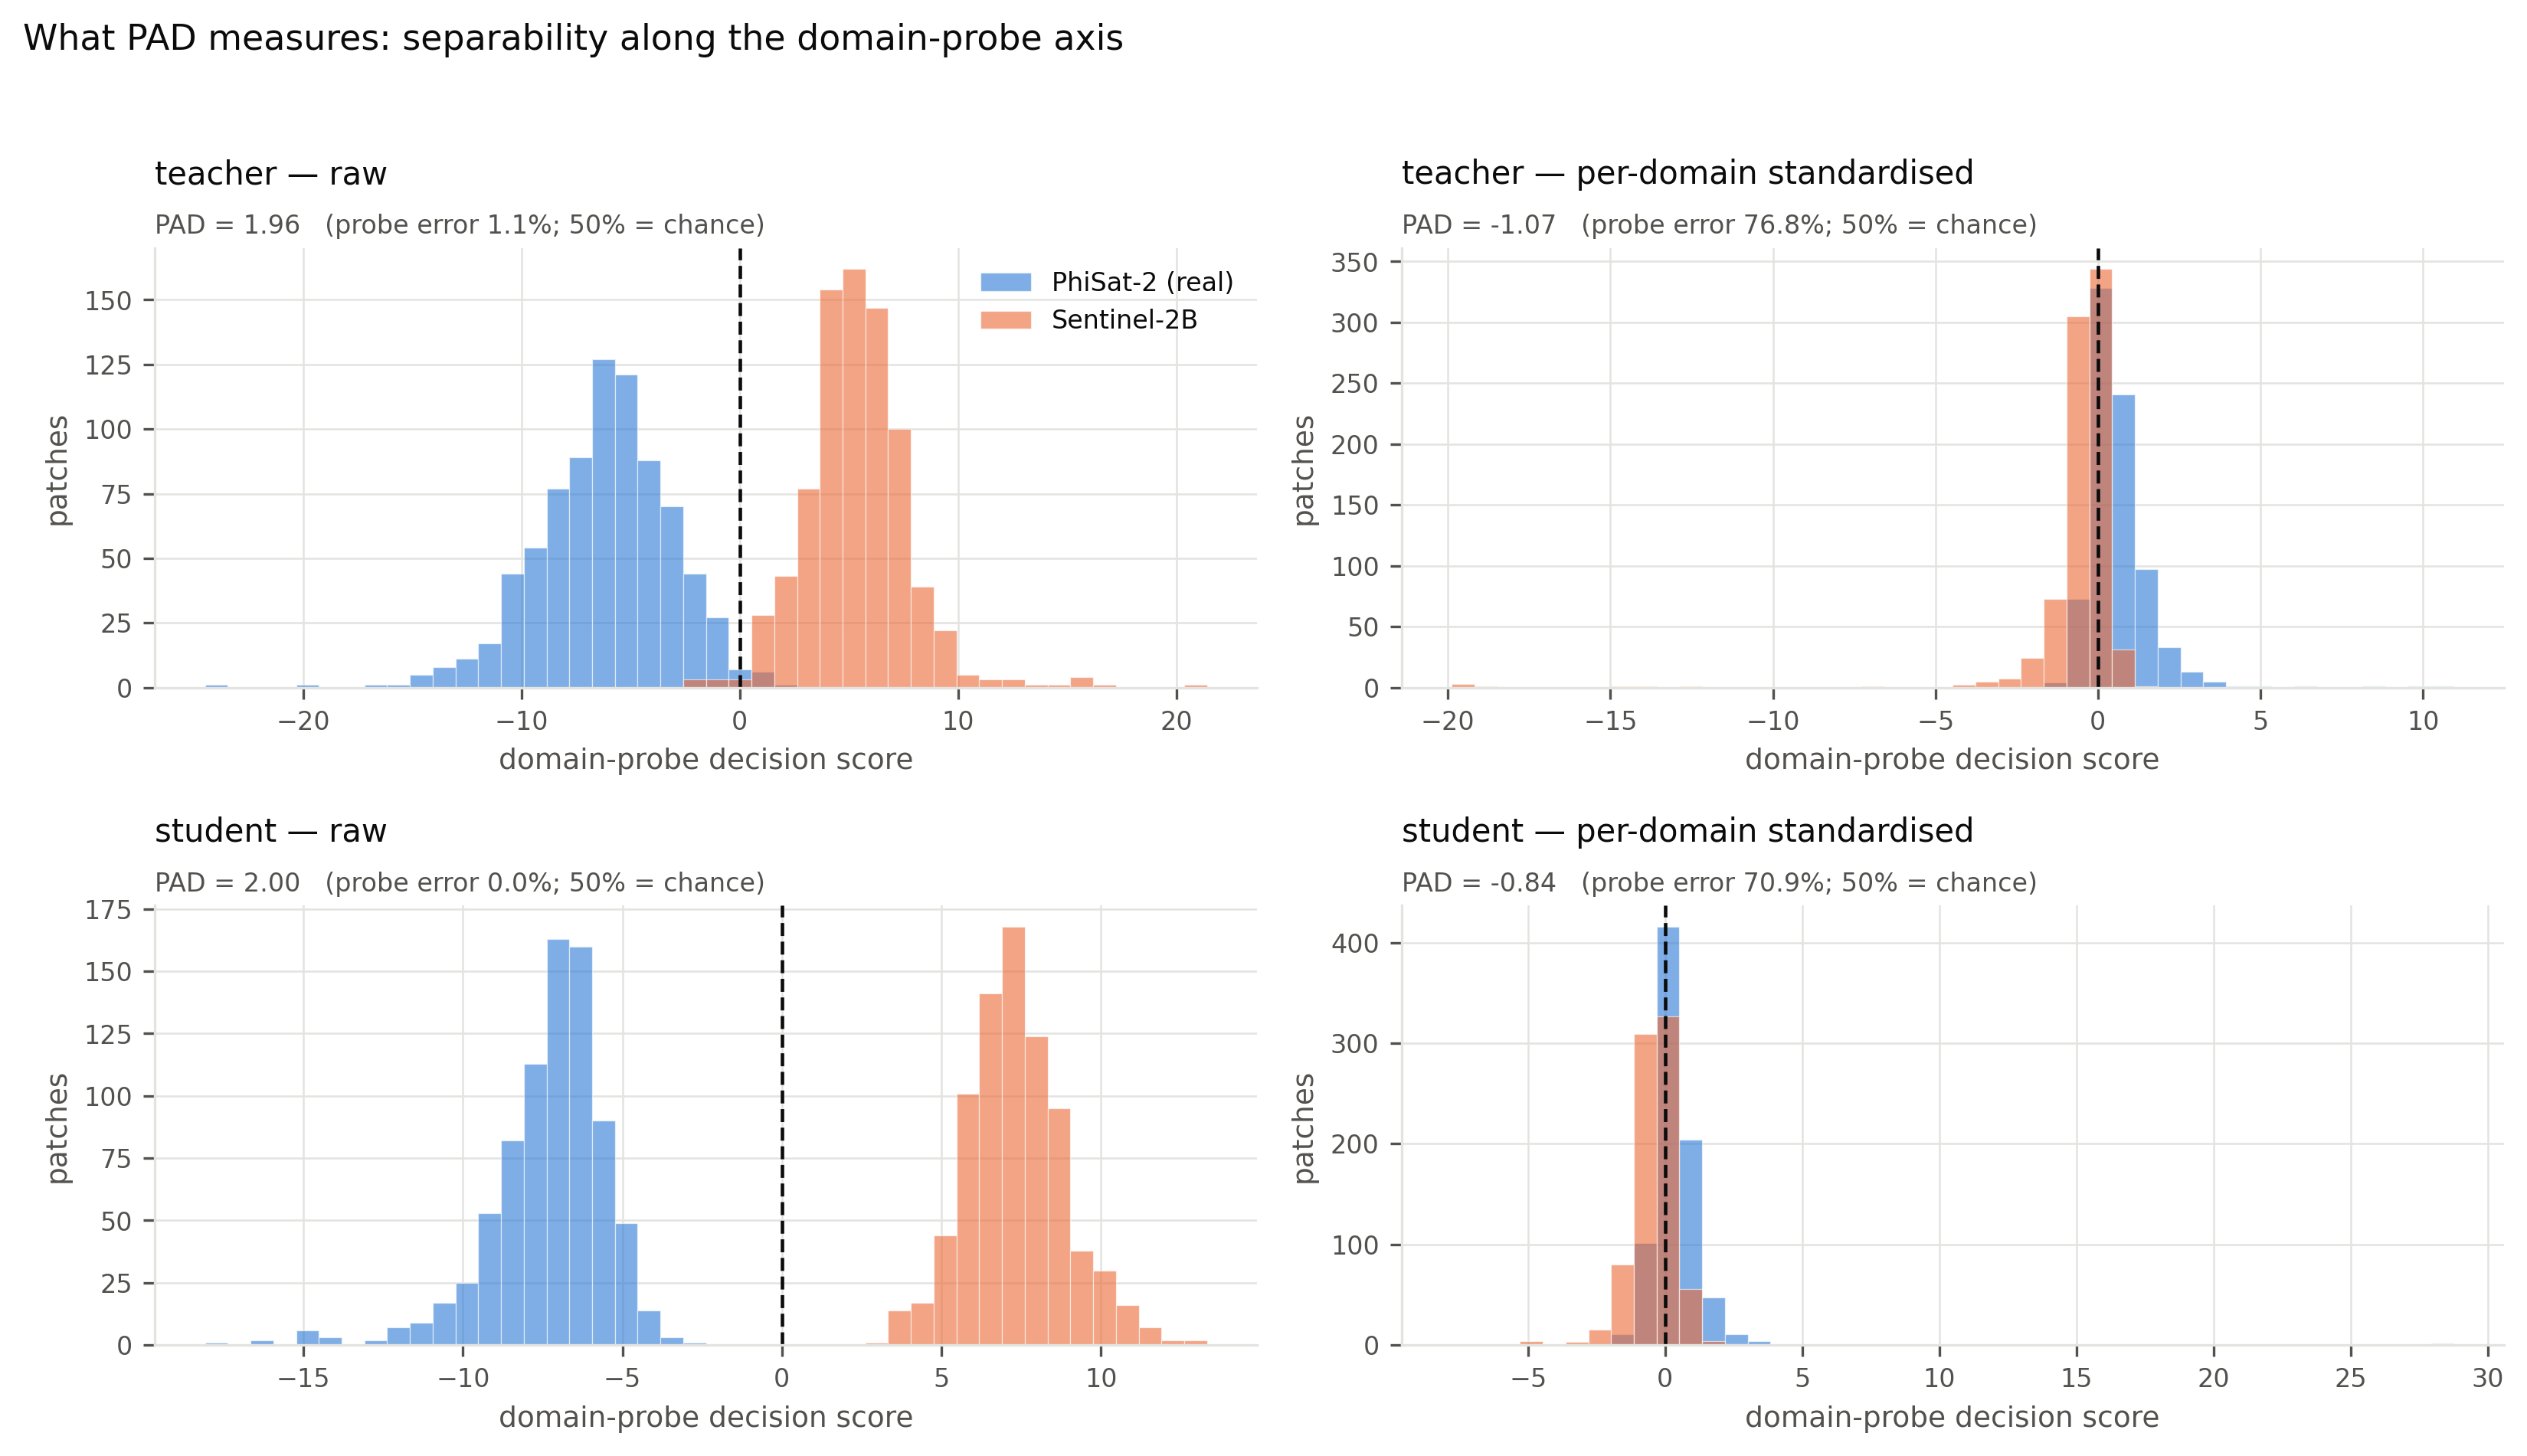
\includegraphics[width=\textwidth]{figures/fig_pad_decision_scores.png}
    \caption{Distribution of the domain probe's out-of-fold decision score, the quantity from which PAD is computed.
        Separated modes imply a probe that never errs (PAD $\rightarrow 2$); overlapping modes imply chance (PAD $\rightarrow 0$).
        After standardising each domain on its own statistics (right column) the separability vanishes for both models, showing that all of it was per-channel mean and scale, not representational structure.
    }
    \label{fig:pad-decision}
\end{figure}

This result should be stated precisely.
With a domain-specific normalization, the encoder is domain-adaptive rather than domain-invariant: the convolutional weights are shared, the normalization statistics are not, and the target-sensor branch has to be selected at inference.
The defensible claim is therefore that after a per-domain normalization, the structure learned on the source sensor is $97\%$ readable on the target one.
That is weaker than a single sensor-agnostic encoder, but it is the property that an on-board deployment actually requires, since the acquiring instrument is always known.

\section{Distillation Against a Supervised Baseline (RQ3)}
\label{sec:rq3-results}

Sensor adaptivity is only useful if it buys an accuracy that a simpler method would not.
Our control is a student of identical architecture, trained directly on labelled $\Phi$-sat-2 with no teacher, no second sensor and no distillation, and holding constant the split, the normalization, the augmentation, the task loss, the optimiser, the schedule and the early-stopping criterion (Table~\ref{tab:hyperparameters}).

At a budget of $10{,}000$ labelled patches the distilled student reaches $0.4607$ best validation mIoU against the baseline's $0.3989$, a margin of $0.0618$ (Table~\ref{tab:main-results}).
Figure~\ref{fig:dsbn-vs-baseline} shows the shape of that margin: the baseline is ahead for roughly the first twenty-five epochs, then the two curves cross, and the distilled run separates and keeps climbing after the baseline has flattened.
Averaged over the $71$ epochs the two runs share, the distilled student leads by $0.0161$ mIoU and is ahead in $49$ of them.

\wip[Settle the framing of the late overtake against the curves.]{%
    To write: an interpretation of \emph{why} the distilled run overtakes late rather than early.
    These runs do not establish the mechanism.
    The candidate explanations are that the teacher's signal becomes most useful once the student has enough capacity committed to the easy classes, or simply that the two-branch arm sees twice the supervision per epoch and therefore trails on wall-clock but not on epochs.
}

The distilled run had not converged.
Its best epoch is the $89$th of the $101$ it ran, and it exhausted the full budget without ever triggering the early stopping, so $0.4607$ should be read as a lower bound on what this configuration reaches.
The baseline, by contrast, early-stopped at epoch $80$.

The per-class results (Figure~\ref{fig:per-class}) show that the gain is a broad one, and not concentrated in a single class.
Distillation is ahead on nine of the eleven classes, most markedly on mangroves ($+0.144$), grassland ($+0.135$), moss/lichen ($+0.115$), tree cover ($+0.100$) and cropland ($+0.099$).
It is behind on permanent water ($-0.019$) and level on shrubland ($-0.002$).
The frequency-weighted IoU moves in the same direction as the macro average ($0.523$ against $0.454$), so this result is not an artefact of the rare-class weighting introduced in Section~\ref{sec:configuration}.

\wip[Decide how much weight the two classes where the baseline wins deserve.]{%
    To write: the per-class discussion.
    Permanent water is the only class where the undistilled baseline is meaningfully ahead ($-0.019$), with shrubland level, and it is spectrally distinctive and not rare enough for the class weighting to be doing the work.
    This needs a sentence on whether that pattern is meaningful, or whether it sits within the per-class noise of a single seed.
}

Two costs qualify this result.
The distillation requires $7.9$ minutes per epoch against the $3.3$ of the baseline, which is a factor of $2.4$, and it is dominated by the forward pass of the frozen teacher and by the second student branch.
At a fixed compute budget rather than a fixed epoch count, the comparison would therefore be much closer.
Separately, the teacher reaches $0.6351$ mIoU on Sentinel-2 while the student reaches $0.4454$ on $\Phi$-sat-2, so roughly $0.19$ mIoU of the teacher--student gap remains unclosed.
That residual is a compression gap rather than a domain gap, since Section~\ref{sec:rq2-results} shows that the student performs almost identically on the two sensors, so what separates it from the teacher is its capacity and its initialisation.

\begin{table}[htbp]
    \centering
    \label{tab:main-results}
    \begin{tabular}{llccc}
        \toprule
        Labels                                                        & Method              & Val.\ mIoU        & Test mIoU         & Cost (h)       \\
        \midrule
        $10{,}000$                                                    & KD + DSBN           & $\mathbf{0.4607}$ & $\mathbf{0.4454}$ & $13.3$         \\
        $10{,}000$                                                    & Supervised baseline & $0.3989$          & $0.3782$          & $\mathbf{4.4}$ \\
        \addlinespace
        $1{,}000$                                                     & KD + DSBN           & $0.2679$          & $0.2635$          & $2.2$          \\
        $1{,}000$                                                     & Supervised baseline & $\mathbf{0.2916}$ & $\mathbf{0.2707}$ & $\mathbf{0.6}$ \\
        \midrule
        \multicolumn{2}{l}{TerraMind teacher (Sentinel-2, reference)} & ---                 & $0.6351$          & ---                                \\
        \bottomrule
    \end{tabular}
    \caption{Main results on the LULC task.
        Validation mIoU is the best epoch, on the fixed $1{,}000$-patch validation split shared by every run; because the splits are nested prefixes of one shuffled ordering, the two label budgets are evaluated on the identical patches.
        Test mIoU is on the full $25{,}323$-patch test split.
        Cost is total wall-clock for the run.
    }
\end{table}

Both test scores in Table~\ref{tab:main-results} are measured on the full $25{,}323$-patch split.
The $10{,}000$-label baseline was originally evaluated on a $997$-patch subset, before the evaluation split was decoupled from the training budget (Section~\ref{sec:measurement-pitfalls}); its stored checkpoint was re-evaluated on the full split for this table, which moved its score from $0.3902$ to $0.3782$ and required no retraining.
The size of that shift is worth noting on its own: the same frozen teacher scores $0.5788$ on the $997$-patch subset and $0.6351$ on the full split, so subset-to-subset differences of this magnitude are not negligible at all, and no number coming from the two evaluation regimes should be compared directly.

\begin{figure}[htbp]
    \centering
    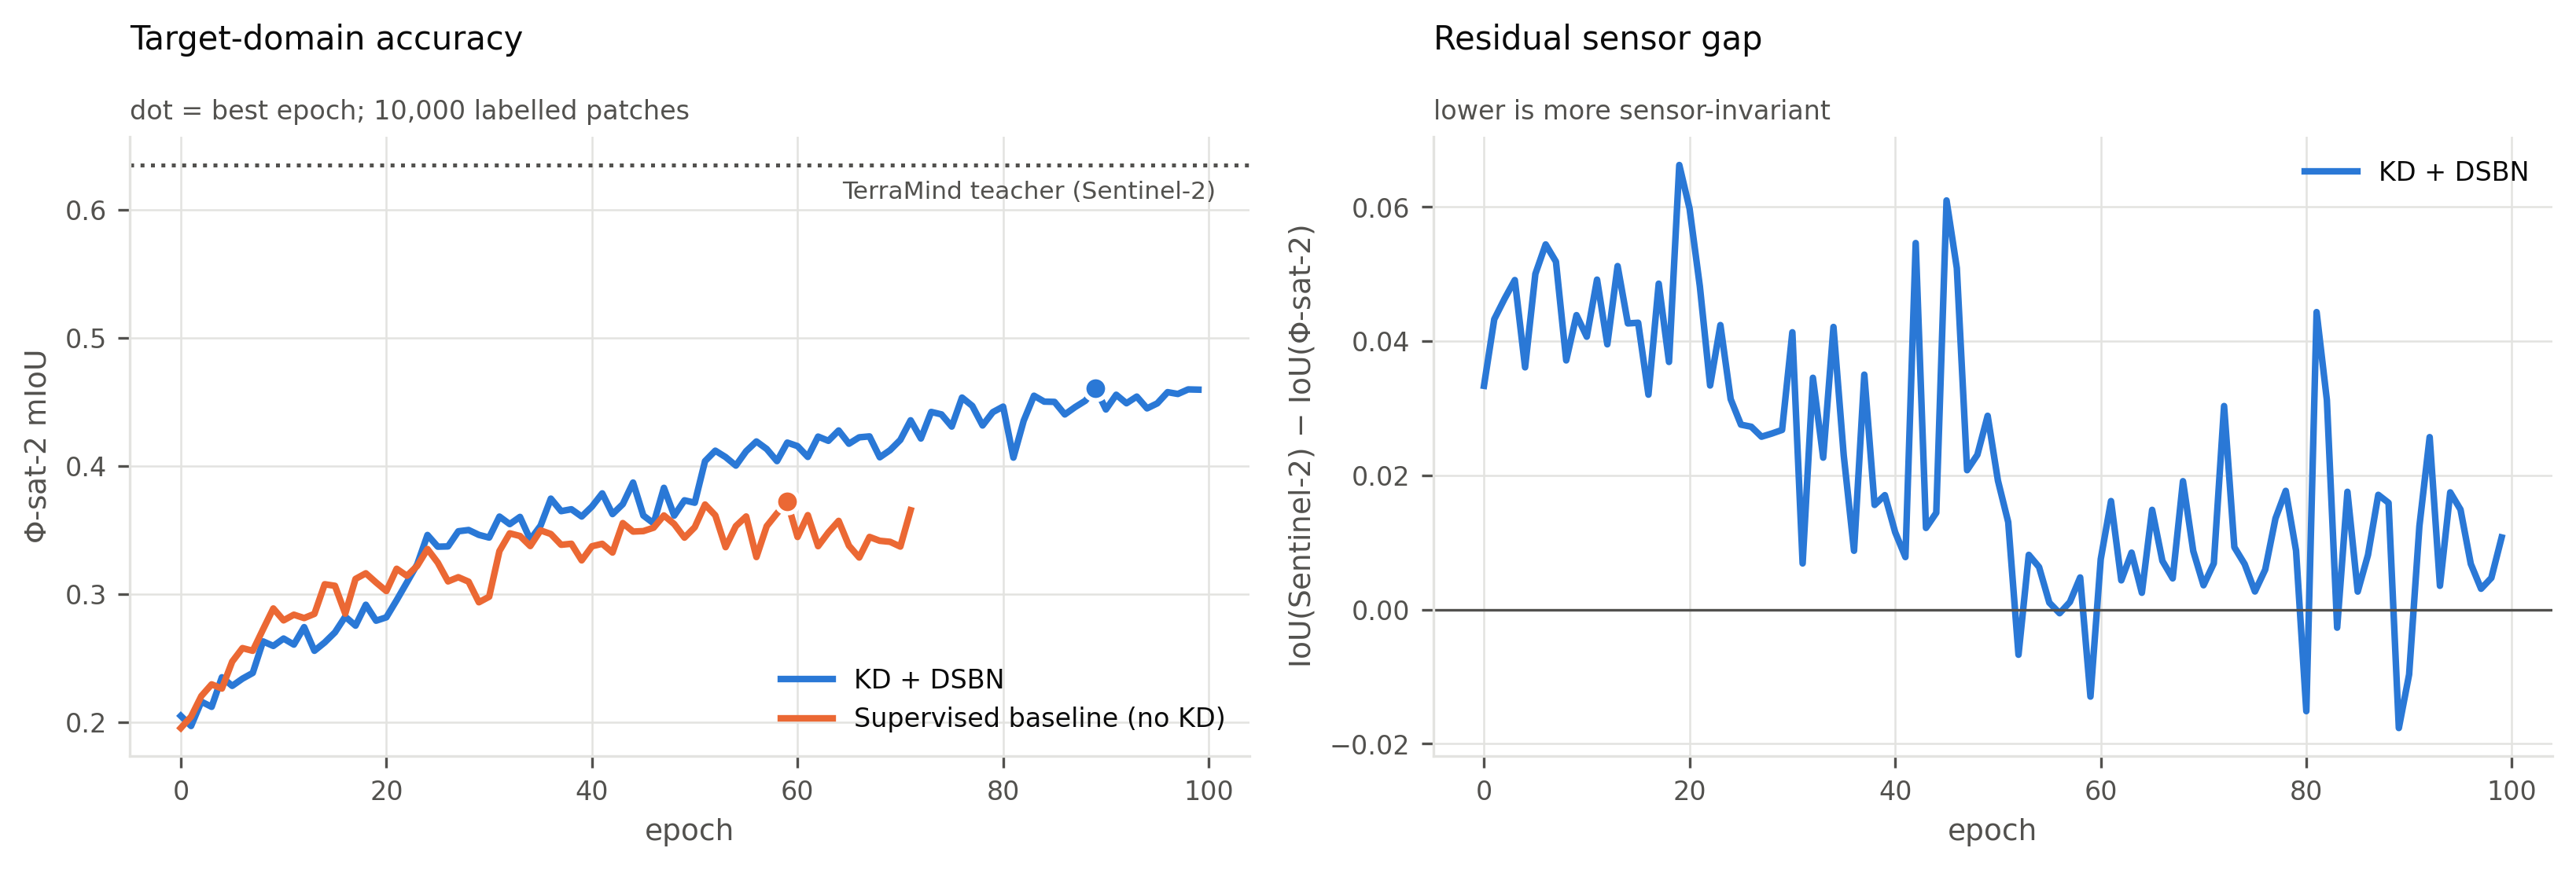
\includegraphics[width=\textwidth]{figures/fig_dsbn_vs_baseline.png}
    \caption{Left: $\Phi$-sat-2 validation mIoU over training at $10{,}000$ labelled patches, with the best epoch marked; the dotted line is the teacher's Sentinel-2 accuracy.
        Right: the residual accuracy difference between the two sensors for the distilled student, which crosses zero around epoch $55$ and oscillates about it thereafter.
    }
    \label{fig:dsbn-vs-baseline}
\end{figure}

\begin{figure}[htbp]
    \centering
    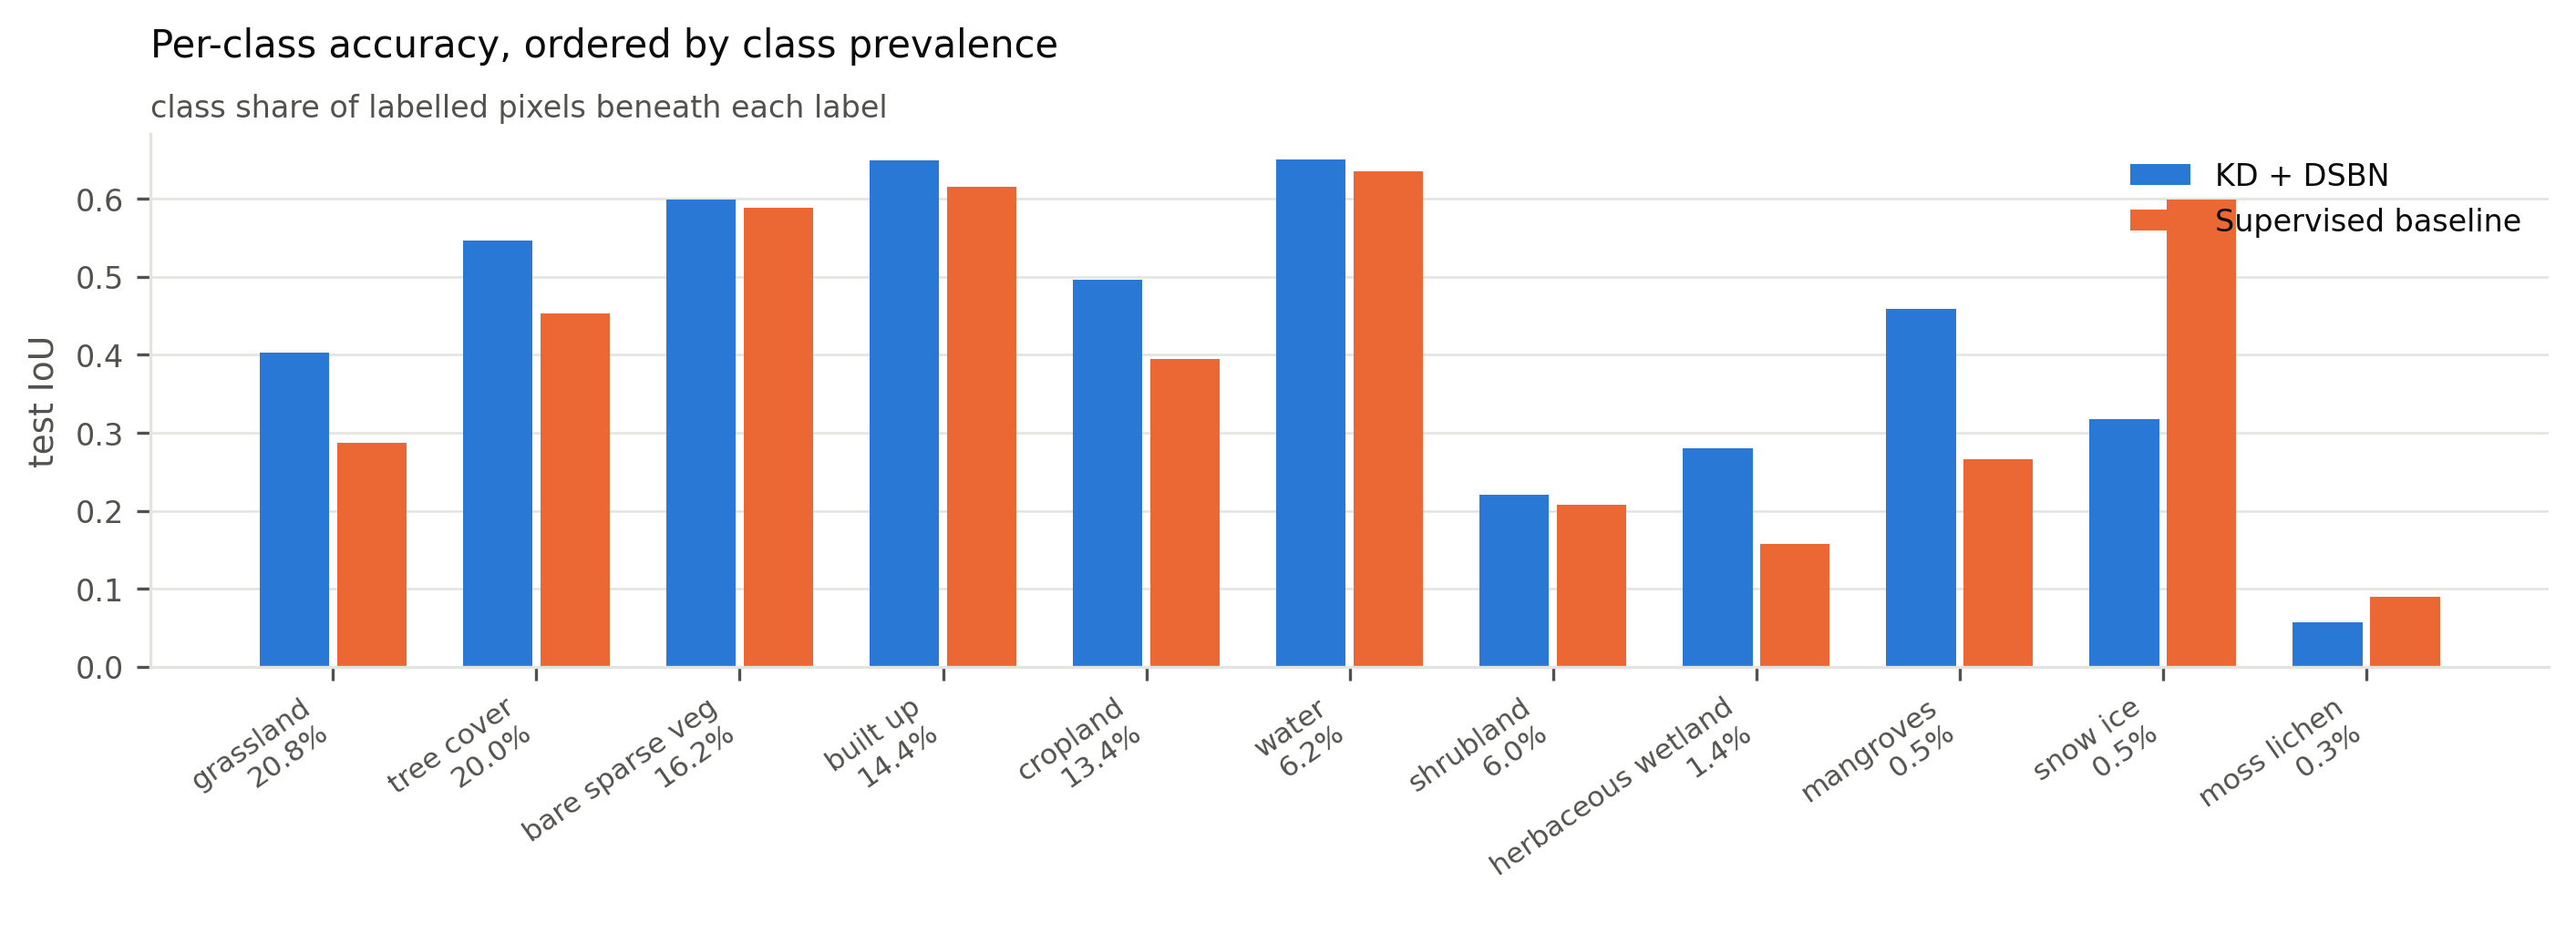
\includegraphics[width=\textwidth]{figures/fig_per_class_dsbn.png}
    \caption{Per-class test IoU at $10{,}000$ labelled patches, ordered by class prevalence, with each class's share of labelled pixels beneath its label.
        Neither model leaves any class unlearned, which unweighted cross-entropy did for four of them (Section~\ref{sec:configuration}).
    }
    \label{fig:per-class}
\end{figure}

\section{Advantage Reversal on Small Label Budget}
\label{sec:label-crossover}

KD and UDA are usually motivated by a label scarcity in the target domain~\cite{kouw2019introductiondomainadaptationtransfer}, so we would expect the advantage above to grow as the target labels are removed, however the opposite is observed.
At $1{,}000$ labelled patches the supervised baseline is ahead by every measure: best validation mIoU $0.2916$ against $0.2679$, test mIoU $0.2707$ against $0.2635$, and on matched epochs the distilled student leads in only $8$ of the $58$ epochs both runs share.
It also does so at roughly a third of the cost, and this even though the distilled run had the larger budget available to it: it used its full hundred epochs without ever triggering the early stopping, while the baseline stopped at sixty-seven.
Figure~\ref{fig:label-crossover} shows the crossover; both budgets are evaluated on the identical fixed $1{,}000$-patch validation split, so the two points are directly comparable.

The reversal is consistent across every measure reported (best validation mIoU, test mIoU, and the epoch-by-epoch lead), but the two ends of the crossover are not equally well resolved.
At $10{,}000$ labels the margin ($0.0543$ validation mIoU) is larger than the epoch-to-epoch variance noted at the start of this chapter; at $1{,}000$ labels it is not ($0.0237$ validation, $0.0072$ test), and the baseline's advantage at the small budget therefore rests mainly on the consistency of the epoch-by-epoch lead, not on the size of the final gap.
Replication across seeds is required before the small-budget end of the crossover can be treated as established, and that is the appropriate reading of it here.
A plausible reading is that the distilled configuration carries substantially more machinery, which is a second forward pass, doubled normalization parameters, and a distillation term pulling toward a teacher that is itself imperfect at $0.5788$ mIoU, and that below a certain label threshold, the cost of all this machinery exceeds the value of the teacher's signal.
This is offered as a hypothesis: with two budgets the crossing point is bracketed but not located, and intermediate budgets would be required to characterise it.

\begin{figure}[htbp]
    \centering
    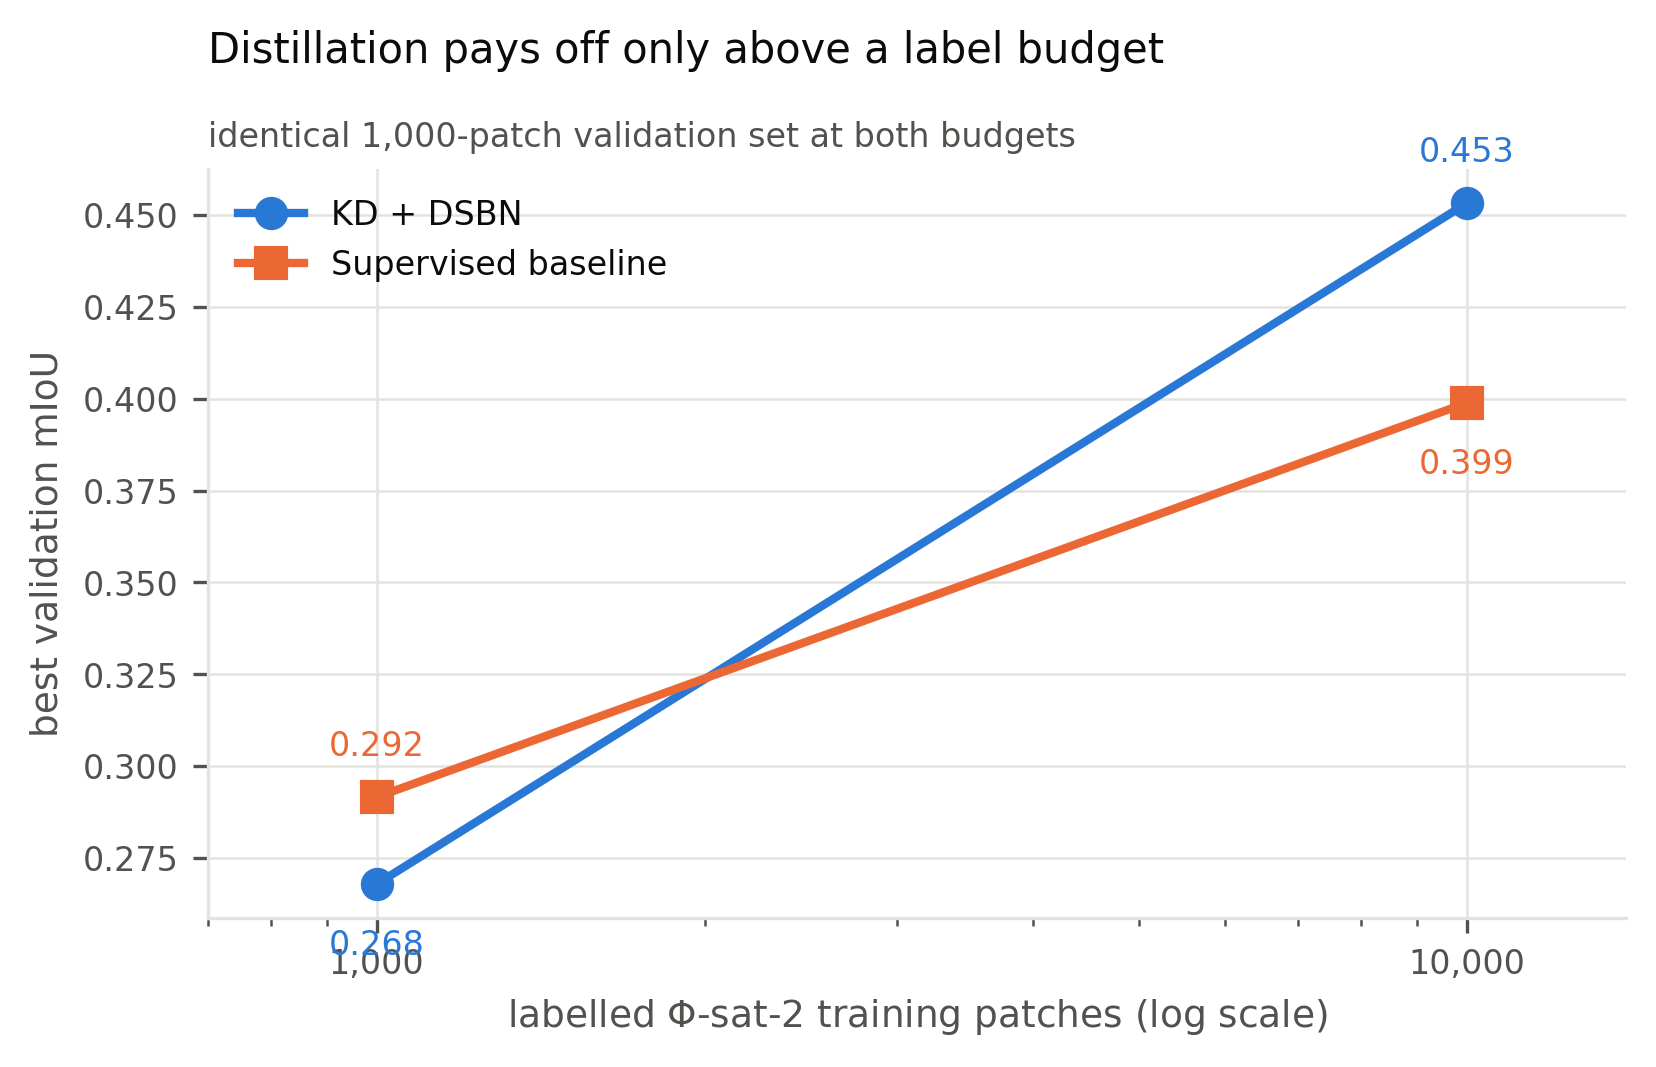
\includegraphics[width=0.72\textwidth]{figures/fig_label_crossover.png}
    \caption{Best validation mIoU against labelled training budget.
        The two methods cross: distillation is worse at $1{,}000$ labelled patches and better at $10{,}000$.
        Both budgets share the same fixed validation split.
    }
    \label{fig:label-crossover}
\end{figure}

\section{Discussion}
\label{sec:discussion}

\subsection{Domain-specific normalization contribution}

The improvement brought by the domain-specific normalization is larger than what a pure domain-alignment effect would predict, and its shape is informative: the accuracy on the source sensor improved by a margin similar to the one on the target ($+0.116$ against $+0.185$ test mIoU relative to the preceding configuration).
A mechanism that only aligned domains should have improved the target branch alone.
The most likely explanation is the train/test normalization inconsistency described in Section~\ref{sec:configuration}: the prior configurations were evaluated through a normalization path that the encoder had never been optimised under, which depressed the two branches at once.
On that reading, part of what is reported here as a domain-adaptation gain is the repair of a latent defect in the two-branch training scheme.
That caveat does not diminish the practical result, but it does bear on how much of it should be attributed to DA.

\subsection{Measurement pitfalls}
\label{sec:measurement-pitfalls}

Two artefacts we encountered during this work are worth recording, since both of them would silently corrupt a comparison of exactly this kind.

First, the macro-averaged mIoU implemented by standard libraries excludes classes with zero union from its average, so its denominator depends on which classes a given model happens to predict.
Where a rare class is absent from a small evaluation split, two models are then averaged over a different number of classes and their mIoU values are simply not comparable.
This effect inflated an apparent advantage by roughly a factor of three in an early version of the label-budget experiment.
All results in this chapter are reported on a fixed denominator over all eleven classes.

Second, and relatedly, an evaluation split sized as a fixed fraction of the training split makes a label-scarcity study vary its measurement and its treatment at the same time.
At the smallest budget, this left us with one hundred evaluation patches, in which the rarest class does not occur at all.
We therefore hold the evaluation splits fixed and independent of the training budget throughout.

\subsection{Limitations}
\label{sec:limitations}

All experiments use at most $10{,}000$ of the $202{,}582$ available training patches, under $5\%$, so the crossover of Section~\ref{sec:label-crossover} is characterised entirely within the low-data regime, and the ranking at full scale is untested.
Single seeds are used everywhere except the degradation-ladder evaluation of Section~\ref{sec:ladder-results}, so apart from that section no result in this chapter is supported by independent replication; epoch-to-epoch validation variance is of the order of $0.02$ mIoU, and differences below roughly $0.03$, which includes the small-budget end of the crossover in Section~\ref{sec:label-crossover}, are consequently not resolved.
Two further controls are outstanding at the time of writing: a shared-normalization distillation run isolating the contribution of domain-specific normalization (Section~\ref{sec:configuration}), and a recomputation of the invariance measures under shared and per-domain-standardised normalization (Section~\ref{sec:rq2-results}).
The student is trained from a random initialisation because no pre-trained weights exist for this backbone, and this plausibly accounts for a substantial share of the remaining $0.15$ mIoU gap to the teacher, and it confounds any claim that this gap would be attributable to a domain shift.
Finally, the work is scoped to a single sensor pair, so the finding that the gap is radiometric rather than resolution-driven (Section~\ref{sec:rq1-results}) should not be generalised beyond it.

\subsection{Interpretation of the flood-robustness result}
\label{sec:discussion-comparison}

\wip{The flood-segmentation evaluation is only partially complete at the time of writing, and the scope of what follows should be read accordingly.
    The robustness assessment across the simulated degradation ladder (Section~\ref{sec:ladder-results}) covers TerraMind, in both frozen and fine-tuned configurations, and the distilled student; the supervised U-Net baseline has not been run across the ladder, so no statement is yet possible about whether distillation changed flood-task robustness relative to training on the target sensor directly.
    The invariance and label-budget findings above therefore still rest on the LULC task alone, and no claim is made yet about whether they carry over to flood segmentation.
}

The mild flood-IoU degradation observed for the teacher across the simulated degradation ladder (Section~\ref{sec:ladder-results}, at worst $-0.152$ IoU under full-severity noise and $-0.008$ under full-severity blur) is not unique to this thesis.
Du et al.~\cite{du2025onorbitdemonstrationgeospatialfoundation} independently report that flood detection was anomalously robust to the sensor domain gap on Kanyini, in contrast to an approximately $47\%$ drop in cloud-detection performance on the same platform.
Two independent studies therefore observe the same pattern, and a plausible explanation is that the strong near-infrared absorption contrast of water survives the sensor noise and the band mismatch much better than the texture-dependent and boundary-dependent cues that cloud detection or general land-cover classification rely on.
Flood segmentation may then understate the severity of the domain-gap problem, and this is part of why we adopted the LULC task as the primary benchmark.

\subsection{Positioning with \texorpdfstring{$\Phi$}{Phi}satNet}

$\Phi$satNet (Section~\ref{sec:phisatnet-background}) reports that a purpose-built, non-transformer model trained from scratch on a mission-specific corpus matches or exceeds unconstrained transformer-based GeoFMs on several on-board tasks~\cite{phisatnet}.
This raises a reasonable objection: if a bespoke lightweight model already performs well without any of the machinery developed here, what is gained by adapting TerraMind instead?

The results of Section~\ref{sec:label-crossover} sharpen that question without settling it.
The answer this thesis offers is a label-efficiency bet: that a large-scale multi-modal pre-training generalises to new $\Phi$-sat-2 tasks with fewer labels than a narrower and curated pre-training suite requires.
The crossover we measure here shows that such a bet is budget-dependent, in a way that has to be quantified rather than assumed.
A matched few-shot comparison against $\Phi$satNet on a shared task and label budget remains the appropriate test and has not been run.

\subsection{Practical recommendations}

Three recommendations follow.
First, the missions intended to host on-board foundation models should prioritise collecting co-registered calibration data across the sensor pair the mission needs to bridge, and this early in their operational life, since this is what made the measurements of this chapter possible at all.
Second, where the deployed sensor is known at inference, which on board a satellite it always is, the domain-specific normalization is a very high value-for-effort intervention: it is only a few hundred additional parameters, and it required no change at all to the training objective.
Third, the label budget should be measured before adopting a distillation pipeline, since below the crossover of Section~\ref{sec:label-crossover}, the simpler supervised baseline was both more accurate and roughly three times cheaper.
